\documentclass[letterpaper,landscape]{article}
\usepackage[margin=0pt,tmargin=7ex]{geometry}
\usepackage{graphicx}
\begin{document}

\includegraphics[page=9,angle=180,width=.24\paperwidth]{source.pdf}\hfill
\includegraphics[page=8,angle=180,width=.24\paperwidth]{source.pdf}\hfill
\includegraphics[page=5,angle=180,width=.24\paperwidth]{source.pdf}\hfill
\includegraphics[page=4,angle=180,width=.24\paperwidth]{source.pdf}\\

\vspace{7ex}

\includegraphics[page=12,angle=0,width=.24\paperwidth]{source.pdf}\hfill
\includegraphics[page=13,angle=0,width=.24\paperwidth]{source.pdf}\hfill
\includegraphics[page=16,angle=0,width=.24\paperwidth]{source.pdf}\hfill
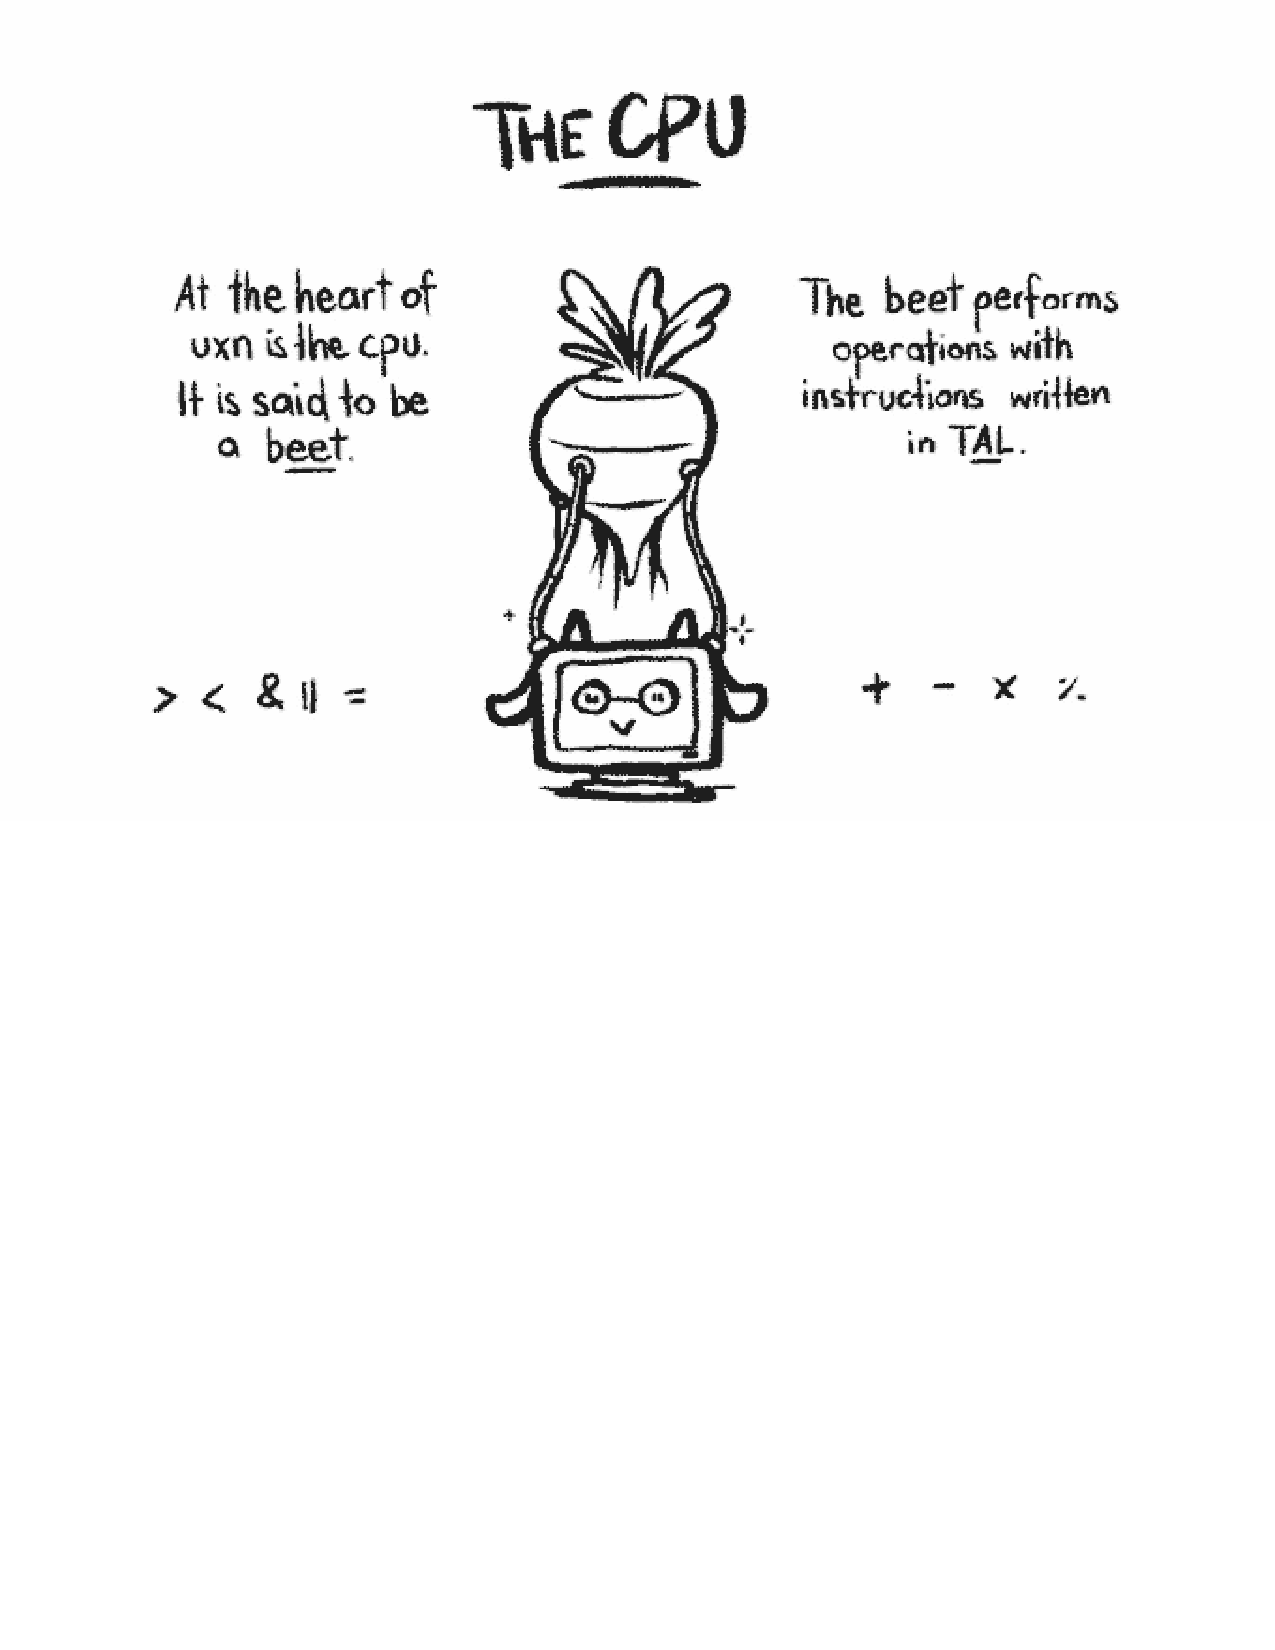
\includegraphics[page=1,angle=0,width=.24\paperwidth]{source.pdf}\hfill

\newpage

\includegraphics[page=3,angle=180,width=.24\paperwidth]{source.pdf}\hfill
\includegraphics[page=6,angle=180,width=.24\paperwidth]{source.pdf}\hfill
\includegraphics[page=7,angle=180,width=.24\paperwidth]{source.pdf}\hfill
\includegraphics[page=10,angle=180,width=.24\paperwidth]{source.pdf}\\

\vspace{7ex}

\includegraphics[page=2,angle=0,width=.24\paperwidth]{source.pdf}\hfill
\includegraphics[page=15,angle=0,width=.24\paperwidth]{source.pdf}\hfill
\includegraphics[page=14,angle=0,width=.24\paperwidth]{source.pdf}\hfill
\includegraphics[page=11,angle=0,width=.24\paperwidth]{source.pdf}\hfill
\end{document}
